In this chapter, we discuss data collected from several simulations run on
our Noisy Complete Components (NCC), Noisy Complete Components with Hubs
(NCCH), and Class-Weighted Barab\'{a}si-Albert (CWBA) models introduced in
Chapter 3. We use these models because they are small-world and have an
intuitive ground truth labeling of vertices. The simple structures of our
models also allow us to test different parameters relating to graph 
structure and examine their effects on prediction accuracies.

For each model, we set a variety of parameters that we want to test.
After constructing the graph, we censor a proportion ($censorP$) of the 
graph, then use a weighted k-nearest neighbors voting (Chapter 5) to solve
a vertex label prediction problem. This process is repeated with the same
parameters $avgRuns$ number of times, and the prediction accuracies
obtained are averaged. We incorporate three different metrics on graphs
(Chapter 4) to our weighted k-nearest neighbors voting algorithm: 
the diffusion state distance (DSD), shortest path distance (SPD), and
resistance distance (RD).


\section{Noisy Complete Components (NCC) Graphs}
% Add more?
In this section, we construct NCC graphs (Chapter 3) and run label 
prediction methods on them.

\subsection{Data Collection}
Our NCC graphs have three input parameters, where $n$ is the number of
vertices in one complete component ($2n$ total vertices), $p$ is the
probability of adding an edge between components, and $q$ is the 
probability of removing an edge within components.

\begin{table}[H]
\centering
\begin{subfigure}[h]{0.4\linewidth}
\begin{tabular}{|l|l|}
\hline
$n$ & $250$ \\ \hline
$p$ & Range from $0$ to $1$\\ \hline
$q$ & $0.5$\\ \hline
$censorP$ & $0.7$\\ \hline
$avgRuns$ & $10$\\ \hline
\end{tabular}
\caption{Fixed $q$}
\end{subfigure}
\hfill
\begin{subfigure}[h]{0.4\linewidth}
\begin{tabular}{|l|l|}
\hline
$n$ & $250$ \\ \hline
$p$ & $0.5$\\ \hline
$q$ & Range from $0$ to $1$\\ \hline
$censorP$ & $0.7$\\ \hline
$avgRuns$ & $10$\\ \hline
\end{tabular}
\caption{Fixed $p$}
\end{subfigure}%
\caption{Tables of parameter values used in our NCC simulations. The table
on the left shows simulation parameters for a fixed $q$, and the table on
the right shows simulation parameters for a fixed $p$.}
\label{table:NCC-params}
\end{table}

Table \ref{table:NCC-params} shows the parameter values we used in our
simulations. The value of parameter $n$ was set to $250$ because this was a
sufficiently large value to allow us to observe differences in prediction
accuracy. Figure \ref{fig:NCC_n} shows that the parameter $n$ only
increases the precision of the prediction accuracies. The parameters $p$
and $q$ were considered probabilities of adding noise to our models, so we
ran simulations to test the effects of these parameters on prediction
accuracies. Figure \ref{fig:NCC_n}(c) shows a plot of the prediction
accuracies over the range of values for $p$, with a fixed $q=0.5$. Figure
\ref{fig:NCC_fixp} shows a plot of the prediction accuracies over the range
of values for $q$, with a fixed $p=0.5$.

\begin{figure}[H]
\begin{subfigure}[h]{0.5\linewidth}
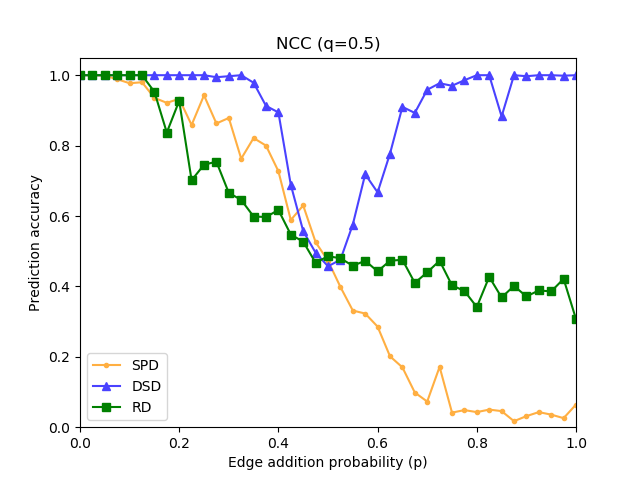
\includegraphics[width=\linewidth]{NCC_fixq_n50.png}
\caption{$n = 50$}
\end{subfigure}
\hfill
\begin{subfigure}[h]{0.5\linewidth}
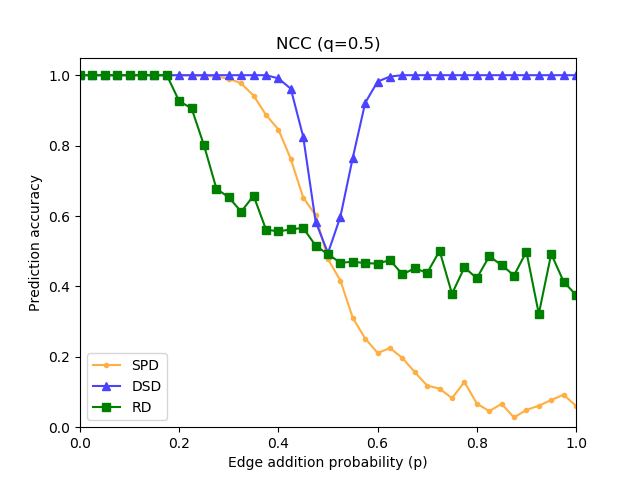
\includegraphics[width=\linewidth]{NCC_fixq_n150.png}
\caption{$n = 150$}
\end{subfigure}
\hfill
\begin{subfigure}[h]{0.5\linewidth}
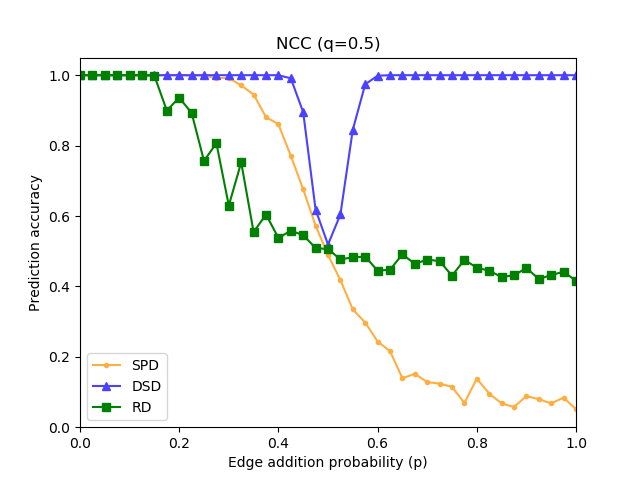
\includegraphics[width=\linewidth]{NCC_fixq_n250.png}
\caption{$n = 250$}
\end{subfigure}
\hfill
\begin{subfigure}[h]{0.5\linewidth}
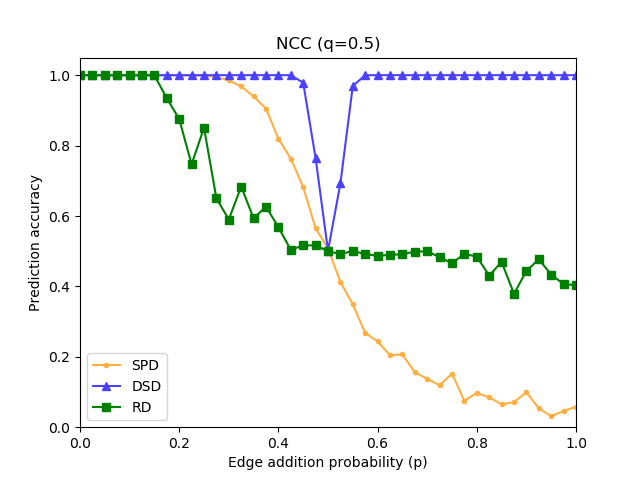
\includegraphics[width=\linewidth]{NCC_fixq_n550.png}
\caption{$n = 550$}
\end{subfigure}%
\caption{These plots show that varying the parameter $n$ in NCC graphs does not change results and a value of $n=250$ will be sufficiently large to observe differences in prediction accuracies. Figure (a) shows that a small value of $n$ may give slightly noisy prediction accuracies due to the smaller number of examples that the prediction accuracies are calculated from.}
\label{fig:NCC_n}
\end{figure}

\begin{figure}[H]
\centering
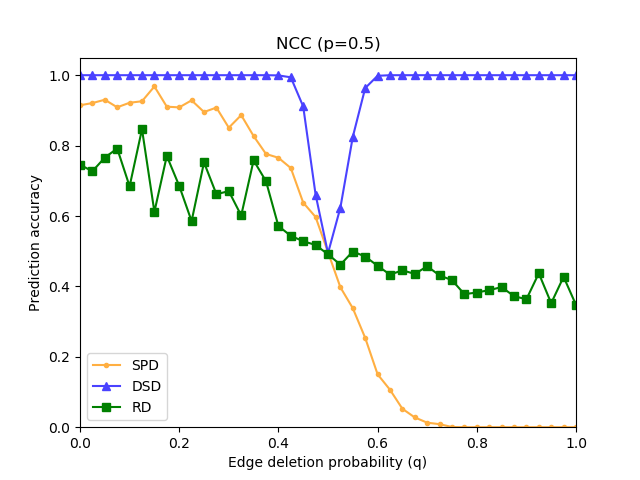
\includegraphics[width=0.8\textwidth]{NCC_fixp.png}
\caption{Plot showing prediction accuracies of the prediction method using the DSD, SPD, and RD metrics. In this simulation, the parameter $p$ was fixed to $0.5$, and $n$ was set to $250$. This plot suggests simulations are symmetric in $p$ and $q$.}
\label{fig:NCC_fixp}
\end{figure}

% Add a part about censorP

\subsection{Analysis}
It is important to note the structure of NCC graphs in extreme cases.
For parameter $p=0$ in NCC graphs (Chapter 3), there is zero probability
of adding edges between components. Since we only consider the largest 
connected component in our analysis, we simply take one of the original components.
If $p=0$ and $q=0$, then we get one complete component. This is not 
interesting, as all prediction methods should attain $100\%$ prediction 
accuracy on these graph. For $p=0$ and $q=1$, we have a set of vertices and no edges. The largest 
connected component would be a single vertex. For $p=1$, there exist edges
from every vertex in one component to every vertex in the other component.
For $p=1$ and $q=1$, we have a complete bipartite graph. We can expect that
a prediction method using the shortest path distance with a small $k$ value
for the $k$-nearest neighbors prediction would result in very poor accuracy
for this method. However, since we have just a binary labeling, these
results can be flipped, making prediction using the inverse of the shortest 
path distance very effective.
With $p=1$ and $q=0$, we have a complete graph where every vertex has equal
same-class degree and different-class degree. This case is not interesting
as all prediction methods would give random results. This leads us to our
next proposition.

\begin{proposition}
For $q = 1 - \frac{mp}{(m-1)}$, NCC graphs are Erd\H{o}s-R\'{e}nyi graphs
with edge probability $p$.
\end{proposition}
\begin{proof}
We know that for NCC graphs (Chapter 3),
$$\E(\deg_{\textit{same}}(u)) = (m-1)(1-q)$$
$$\E(\deg_{\textit{diff}}(u)) = (m)p$$
If $q = 1 - \frac{mp}{(m-1)}$, then we get
$$\E(\deg_{\textit{same}}(u)) = (m-1)(1 - (1 - \frac{mp}{(m-1)})) = mp$$
$$\E(\deg_{\textit{diff}}(u)) = (m)p$$
Thus, we get
$$\E(\deg_{\textit{same}}(u)) = \E(\deg_{\textit{diff}}(u))$$
\end{proof}

The NCC graph with parameters $p$, and $q = 1 - \frac{mp}{(m-1)}$ is expected
to be close to an $(2mp)$-regular graph, where each vertex is expected to 
have the same number of same-class neighbors as different-class neighbors.

The expected number of same-class and different-class neighbors of a vertex
$u$ in an NCC graph corresponds to the expected same-class and 
different-class degrees from Chapter 3. So, from Theorem \ref{thm:ncc_deg}, 
we derive the following result.

\begin{proposition}
For two vertices $u,v$ in an NCC graph,
\begin{enumerate}[(1)]
\item If $u,v$ belong to the same class, they are expected to have 
$$(m-2)(1-q)^2$$ 
common same-class neighbors, and 
$$(m)p^2$$
common different-class neighbors.

\item If $u,v$ belong to different classes, they are expected to have 
$$(2m-2)(1-q)p$$
common neighbors.
\end{enumerate}
\end{proposition}

\begin{proof}
(1) We can see that if $u,v$ belong to the same class, there are $(m-2)$ 
possible same-class vertices that could be common neighbors between them. 
Each of these vertices has a $(1-q)$ probability of being a same-class 
neighbor of $u$ and a $(1-q)$ probability of being a same-class neighbor of 
$v$ (chapter 3). Therefore, we get that the expected number of common same-
class neighbors is $(m-2)(1-q)^2$.

Also, there are $m$ possible different-class vertices that could be common
neighbors between $u$ and $v$. Each of these vertices has a $p$ probability
of being a different-class neighbor of $u$ and a $p$ probability of being a
different-class neighbor of $v$. Therefore, we get that the expected number
of common different-class neighbors is $(m)p^2$.\\

\noindent
(2) If $u,v$ belong to different classes, there are $(2m-2)$ possible 
vertices that could be common neighbors of $u$ and $v$. Without loss of 
generality, each vertex has a $(1-q)$ probability of being a neighbor of $u$
and a $p$ probability of being a neighbor of $v$. Therefore, we get that the
expected number of common neighbors is $(2m-2)(1-q)p$.
\end{proof}

Figure \ref{fig:NCC_n}(c) shows that with a fixed probability of deleting
edges within components of NCC graphs, and a range of probabilities of
adding edges between components of NCC graphs, the label prediction method
using the DSD outperforms the method using SPD and the method using RD.
We can use expected values of same-class degrees (Chapter 3) to reason why
such behavior occurs.

For a fixed $q=0.5$, we can say for any vertex $u$,
$$\E(\deg_{\textit{same}}(u)) = (249)(0.5)$$
$$\E(\deg_{\textit{diff}}(u)) = (250)p$$
We can clearly see that for $p=0.5$, the resulting graph will be random,
having roughly the same number of same-class neighbors as different-class 
neighbors. This explains the near random prediction accuracies when $p$ is
close to $0.5$. However, for $p < 0.5$, we can expect that
$\E(\deg_{\textit{same}}(u)) > \E(\deg_{\textit{diff}}(u))$.
In this case, the prediction method using SPD should predict with high
accuracy, with a sharp decline as the value of $p$ approaches $0.5$. For 
$p > 0.5$, the prediction method using SPD should predict with low 
accuracy, since $\E(\deg_{\textit{same}}(u)) < \E(\deg_{\textit{diff}}(u))$. Figure
\ref{fig:NCC_n}(c) shows this behavior of the prediction method using SPD.

The prediction method using DSD seems only to be affected by the $p$
parameter when it approaches $0.5$, and the graph becomes random. This
behavior can be explained by the fact that the DSD cares about common
neighborhoods when determining similarity, or distance. First we must note
that all vertices in the NCC graph should be very similar to each other,
since they all share the same $\E(\deg_{\textit{same}}(u))$ and
$\E(\deg_{\textit{diff}}(u))$. This means that there is no point in differentiating
between low-degree and high-degree neighborhoods for the NCC graphs.
For $p < 0.5$, we know that $\E(\deg_{\textit{same}}(u)) > \E(\deg_{\textit{diff}}(u))$.
This means that when looking at the neighborhoods of an arbitrary vertex 
$u$, a large number of common neighbors will be shared between vertices
within the same component. Two vertices within the same component will 
share more common neighbors than two vertices in different components. This 
is also true for $p > 0.5$, where 
$\E(\deg_{\textit{same}}(u)) < \E(\deg_{\textit{diff}}(u))$. This means that the DSD
between any two vertices within the same component is expected to be closer
than two vertices in different components for most values of $p$ given $q$ 
is fixed.

% Rewrite when Ch4 written
The prediction method using RD performs the worst of the three metrics.
Since the resistance distance considers the number of short paths between
vertices when calculating distance, we can look at the short paths in NCC
graphs. NCC graphs are very dense in edges, and because of the random
probabilities of adding and deleting edges, it is difficult to obtain a
structured notion of paths in this graph.

A similar analysis can be done for the simulation for a fixed $p=0.5$ over
the range of values for $q$, as shown in Figure \ref{fig:NCC_fixp}.


\section{Noisy Complete Components with Hubs (NCCH) Graphs}
In this section, we construct NCCH graphs (Chapter 3) and run label 
prediction methods on them. We study these graphs in order to determine the
effects of hub vertices on the prediction accuracies of NCC graphs. It is
important to note that the hub vertices in NCCH graphs were labeled 
randomly.

\begin{table}[H]
\centering
\begin{subfigure}[h]{0.4\linewidth}
\begin{tabular}{|l|l|}
\hline
$n$ & $250$ \\ \hline
$p$ & Range from $0$ to $1$\\ \hline
$q$ & $0.5$\\ \hline
\textit{hubs} & $100$\\ \hline
\textit{hubsP} & $0.8$\\ \hline
$censorP$ & $0.7$\\ \hline
$avgRuns$ & $10$\\ \hline
\end{tabular}
\caption{Fixed $q$}
\end{subfigure}
\hfill
\begin{subfigure}[h]{0.4\linewidth}
\begin{tabular}{|l|l|}
\hline
$n$ & $250$ \\ \hline
$p$ & $0.5$\\ \hline
$q$ & Range from $0$ to $1$\\ \hline
\textit{hubs} & $100$\\ \hline
\textit{hubsP} & $0.8$\\ \hline
$censorP$ & $0.7$\\ \hline
$avgRuns$ & $10$\\ \hline
\end{tabular}
\caption{Fixed $p$}
\end{subfigure}%
\caption{Tables of parameter values used in our NCCH simulations. The table
on the left shows simulation parameters for a fixed $q$, and the table on
the right shows simulation parameters for a fixed $p$.}
\label{table:NCCH-params}
\end{table}

\subsection{Data Collection}
We used the same values for similar parameters to the NCC graphs as described in the previous sections. The same process of fixing the parameter $p$ or $q$ in the NCC graphs was used.

The NCCH graphs have two more input parameters, \textit{hubs} and \textit{hubsP}, as
shown in Table \ref{table:NCCH-params}. The \textit{hubs} parameter specifies the
number of hub vertices to add, and the \textit{hubsP} parameter specifies what
proportion of the vertices in the complete components to add edges from each newly added hub vertex. A value of $0.8$ was decided for the \textit{hubsP} 
parameter in order to capture the idea of hub vertices and their large 
degrees. Figures \ref{fig:NCCH_fixq} and \ref{fig:NCCH_fixp} show our 
simulation results.

\begin{figure}[H]
\centering
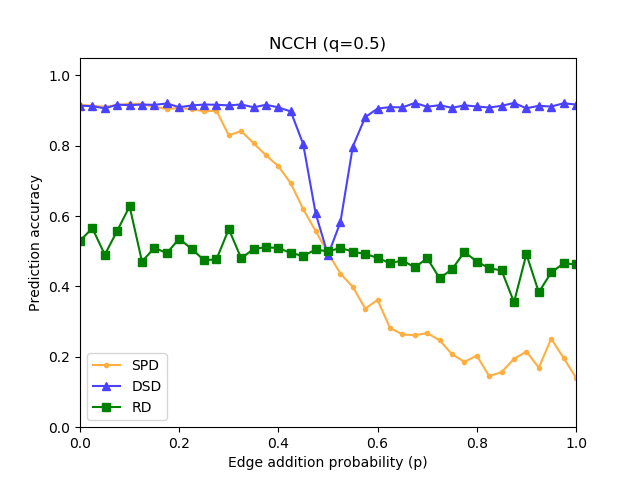
\includegraphics[width=0.7\textwidth]{NCCH_fixq.png}
\caption{Plot showing prediction accuracies of the prediction method using the DSD, SPD, and RD metrics. In this simulation, the parameter $q$ was fixed to $0.5$.}
\label{fig:NCCH_fixq}
\end{figure}

\begin{figure}[H]
\centering
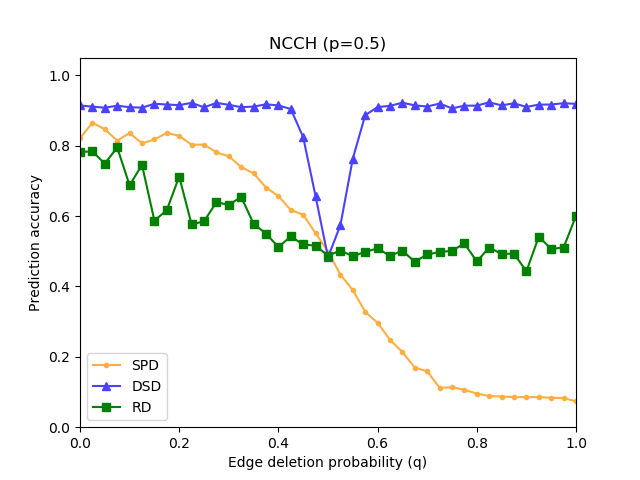
\includegraphics[width=0.7\textwidth]{NCCH_fixp.png}
\caption{Plot showing prediction accuracies of the prediction method using the DSD, SPD, and RD metrics. In this simulation, the parameter $p$ was fixed to $0.5$.}
\label{fig:NCCH_fixp}
\end{figure}

\begin{figure}[H]
\centering
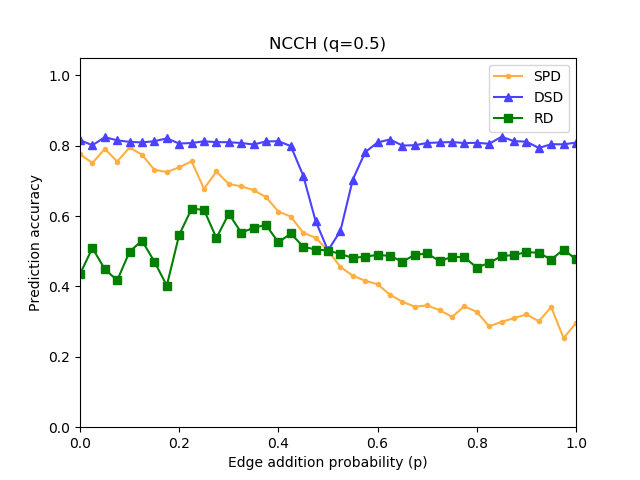
\includegraphics[width=0.8\textwidth]{NCCH_fixq_r300.png}
\caption{Plot showing compressed prediction accuracies for a larger value of the \textit{hubs} parameter. In this simulation, the parameter $q$ was fixed to $0.5$, and \textit{hubs} was set to $300$.}
\label{fig:NCCH_fixq_r300}
\end{figure}

In order to test the effects of the number of hub nodes added, 
prediction accuracies were plotted over the \textit{hubs} parameter. Both 
parameters $p$ and $q$ were set to fixed values such that the prediction
accuracies using DSD, SPD, and RD could be clearly separated. Thus a value
of $p=0.2$ and $q=0.5$ was chosen. These parameters are shown in Table 
\ref{table:NCCH-params-r}.

\begin{table}[H]
\centering
\begin{tabular}{|l|l|}
\hline
$n$ & $250$ \\ \hline
$p$ & $0.2$\\ \hline
$q$ & $0.5$\\ \hline
\textit{hubs} & Range from $0$ to $400$\\ \hline
\textit{hubsP} & $0.8$\\ \hline
$censorP$ & $0.7$\\ \hline
$avgRuns$ & $10$\\ \hline
\end{tabular}
\caption{Tables of parameter values used for our NCCH simulations over the \textit{hubs} parameter.}
\label{table:NCCH-params-r}
\end{table}

\begin{figure}[H]
\centering
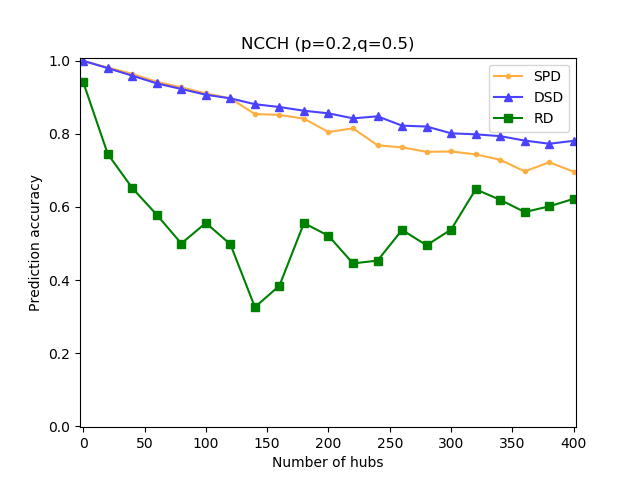
\includegraphics[width=0.8\textwidth]{NCCH_r400.png}
\caption{Plot showing prediction accuracies over the \textit{hubs} parameter. In this simulation, the parameter $p$ was fixed to $0.2$, and $q$ was fixed to $0.5$.}
\label{fig:NCCH_r400}
\end{figure}

\subsection{Analysis}
We can perform a similar analysis to that of the NCC graphs. We can see
in Figures \ref{fig:NCCH_fixq} and \ref{fig:NCCH_fixp} that the shapes of 
the prediction accuracy curves do not change significantly. The main
difference between these plots and the plots for the NCC graphs are that
the plots for NCCH graphs are slightly compressed vertically. This behavior
can be explained by the presence of the hub vertices. Since these hub
vertices are labeled at random, there will always be a proportion of the
vertices in the NCCH graphs that can only be predicted at random. 
Specifically in the case of Figure \ref{fig:NCCH_fixq}, we see that the
prediction accuracies start at $0.9$ rather than $1.0$. If we consider the
number of hub vertices added, $hubs=100$, in relation the the number of
vertices in the NCCH graph, $2n + hubs = 600$, then we can see that since
hub vertices will be predicted at random, we should expect a prediction
accuracy of around $\frac{550}{600} \approx 0.92$. A simulation run with
the parameter $hubs=300$ was run, and shows this idea of compression in
Figure \ref{fig:NCCH_fixq_r300}. The change in the rate of compression can
be seen in Figure \ref{fig:NCCH_r400}.

\section{Class-weighted Barab\'{a}si-Albert (CWBA) Graphs}
In this section, we construct CWBA graphs (Chapter 3) and run label
prediction methods on them. We study the CWBA graphs because they are
scale-free.

\subsection{Data Collection}

\begin{table}[H]
\centering
\begin{subfigure}[h]{0.4\linewidth}
\begin{tabular}{|l|l|}
\hline
$n$ & $1000$ \\ \hline
$m$ & Range from $1$ to $300$\\ \hline
$\rho$ & $2$\\ \hline
$censorP$ & $0.7$\\ \hline
$avgRuns$ & $10$\\ \hline
\end{tabular}
\caption{Fixed $\rho$}
\end{subfigure}
\hfill
\begin{subfigure}[h]{0.4\linewidth}
\begin{tabular}{|l|l|}
\hline
$n$ & $1000$ \\ \hline
$m$ & $300$\\ \hline
$\frac{1}{\rho}$ & Range from $0.05$ to $1$\\ \hline
$censorP$ & $0.7$\\ \hline
$avgRuns$ & $10$\\ \hline
\end{tabular}
\caption{Fixed $\rho$}
\end{subfigure}%
\caption{Tables of parameter values used in our CWBA simulations. The table
on the left shows simulation parameters for a fixed $\rho$, and the table
on the right shows simulation parameters for a fixed $m$ over the inverse of $\rho$.}
\label{table:CWBA-params}
\end{table}

Our CWBA graphs have two input parameters, where $m$ is the minimum vertex
degree, and $\rho$ is the factor of same-class attachment. Table
\ref{table:CWBA-params} shows the parameters used in our simulation. We
also studied the prediction accuracies over $\frac{1}{\rho}$ in order to
study the entire range of values for $\rho$.

\begin{figure}[H]
\centering
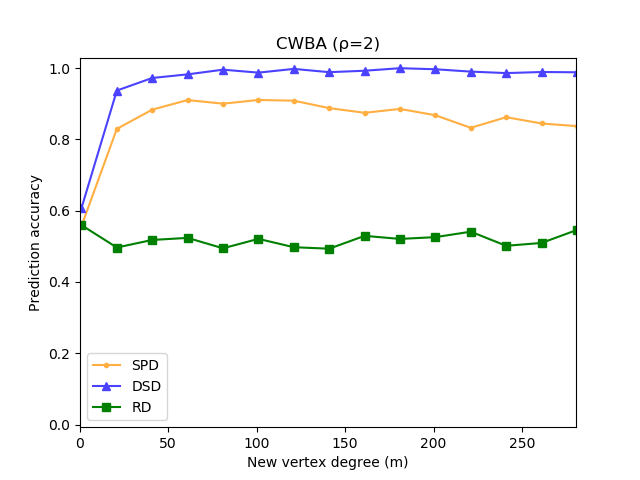
\includegraphics[width=0.8\textwidth]{CWBA_fixrho.png}
\caption{Plot showing prediction accuracies over the $m$ parameter. In this simulation, the parameter $\rho$ was fixed to $2$.}
\label{fig:CWBA_fixrho}
\end{figure}

\begin{figure}[H]
\centering
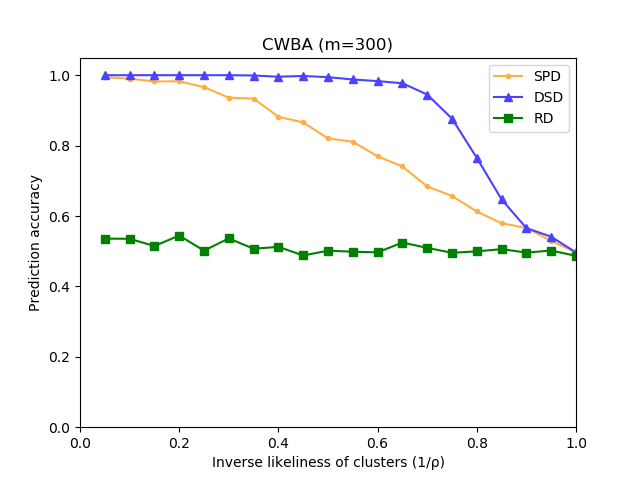
\includegraphics[width=0.8\textwidth]{CWBA_rhoinv.png}
\caption{Plot showing prediction accuracies over the inverse of the $\rho$
parameter. In this simulation, the parameter $m$ was fixed to $300$.}
\label{fig:CWBA_rhoinv}
\end{figure}

\subsection{Analysis}
% Fix when Ch4 done
In our simulations for the CWBA graph, our initial graph is a star $S_m$.
It is important to discuss the extreme cases for CWBA graphs.

\begin{proposition}
When $\rho=1$ for CWBA graphs, we get a randomly labeled scale-free graph.
\end{proposition}
\begin{proof}
We note that when $\rho=1$, the probability of drawing an edge to a vertex $u$ in the CWBA process (Chapter 3) becomes
\[
  p_u = \begin{cases}
    \frac{\deg(u)}{w} &: u \in S_l\\
    
    \frac{\deg(u)}{w} &: u \in (V_G - S_l)\\
  \end{cases}
\]
where
\[
  w = \sum_{v \in S_l}\deg(v) + \sum_{v \in (V_G - S_l)}\deg(v)
\]

We can clearly see that with $\rho=1$, there is no preference in attachment
based on the label, so all vertices are preferentially connected based on
the degree of vertices.
\end{proof}

For $\rho=0$, we can see that vertices with opposite label would only be
considered for attachment, and the opposite would be true for extremely 
high values of $\rho$.

Figures \ref{fig:CWBA_fixrho} and \ref{fig:CWBA_rhoinv} show DSD aids in
predicting more accurately than the other two metrics. Figure 
\ref{fig:CWBA_rhoinv} fixes a value for the parameter $m = 300$ and shows
prediction accuracies over the entire range of values for the $\rho$
parameter. The figure illustrates that when the same-class preferential
attachment factor $\rho$ is $1$, the resulting CWBA graph is random, since
there is no notion of preferential attachment for $\rho=1$. However, for
$\rho > 1$, drawing same-class edges are preferred and this results in a
sharp increase in accuracy for the prediction method using DSD, while the
method using SPD increases at a linear rate. We must note that the 
parameter for minimum vertex degree, $m$, was fixed at $m=300$, so the
resulting CWBA graph is fairly dense. Figure \ref{fig:CWBA_fixrho} shows 
that increasing the parameter $m$ will not change prediction accuracies for
$\rho > 1$, as all of the curves in the plot level out very quickly.

\section{Overall Findings}
After analyzing the results of our simulations, we have found that the 
shortest path distance (SPD) works well with few paths between clusters. The
diffusion state distance (DSD) works well in general as long as neighborhoods
can be distinguished. This can be seen from the NCC and NCCH graph 
simulations. The resistance distance (RD), however, does not seem to work
very well with our simulations, and seems to work best on very sparse graphs.